% Created 2020-09-14 Mon 14:54
% Intended LaTeX compiler: lualatex
\documentclass[11pt]{article}
\usepackage{graphicx}
\usepackage{grffile}
\usepackage{longtable}
\usepackage{wrapfig}
\usepackage{rotating}
\usepackage[normalem]{ulem}
\usepackage{amsmath}
\usepackage{textcomp}
\usepackage{amssymb}
\usepackage{capt-of}
\usepackage{hyperref}
\usepackage{tabularx}
\usepackage{etoolbox}
\makeatletter
\def\dontdofcolorbox{\renewcommand\fcolorbox[4][]{##4}}
\AtBeginEnvironment{minted}{\dontdofcolorbox}
\makeatother
\usepackage[newfloat]{minted}
\author{Mark Armstrong}
\date{\today}
\title{The Boom hierarchy in Scala}
\hypersetup{
   pdfauthor={Mark Armstrong},
   pdftitle={The Boom hierarchy in Scala},
   pdfkeywords={},
   pdfsubject={A brief background on the Boom hierarchy family of datatypes, followed by a (in the end, flawed) implementation in Scala.},
   pdfcreator={Emacs 27.0.90 (Org mode 9.3.8)},
   pdflang={English},
   colorlinks,
   linkcolor=blue,
   citecolor=blue,
   urlcolor=blue
   }
\begin{document}

\maketitle
\tableofcontents


\section{Introduction}
\label{sec:orgce555ad}
These notes were created for, and in some parts \textbf{during},
the lecture on September 14th and the following tutorials.

:TODO: There are still some parts without commentary or with incomplete examples.
They will be fixed, and another announcement made when this file is complete.

\section{The (extended) Boom hierarchy\hfill{}\textsc{theory}}
\label{sec:orgb792d1b}
\subsection{Introduction}
\label{sec:org1a6ed54}
We begin with some (relatively brief) theory.

The Boom hierarchy was introduced
by \href{https://www.kestrel.edu/people/meertens/publications/}{Lambert Meertens} in
\href{https://www.kestrel.edu/people/meertens/publications/papers/Algorithmics.pdf}{Algorithmics — Towards programming as a mathematical activity};
Meertens attributes the concept to H. J. Boom, hence the name.

The Boom hierachy is a family of data structures
—namely trees, lists, bags and sets—
for which we have an \texttt{empty} value and can construct \texttt{singleton} values,
and which include a \texttt{join} operation
(for sets and bags also called \texttt{union}, written \texttt{∪},
and for lists also called \texttt{append}, \texttt{++}).

:TODO:
Notation:
\begin{itemize}
\item \texttt{[]} for empty,
\item \texttt{[a]} for a singleton containing \texttt{a},
\item \texttt{++} for append.
\end{itemize}

The basic idea of the hierarchy is that
\begin{itemize}
\item sets have a \texttt{join} operation which
\begin{itemize}
\item has an identity \texttt{A ∪ ∅ = A},
\item is idempotent \texttt{A ∪ A = A},
\item is commutative \texttt{A ∪ B = B ∪ A}, and
\item is associative \texttt{A ∪ (B ∪ C) = (A ∪ B) ∪ C}. Then,
\end{itemize}
\item bags are like sets, except the \texttt{join} operation is not idempotent,
\item lists are like bags, except the \texttt{join} operation is not commutative, and
\item trees are like lists, except the \texttt{join} operation is not associative.
\end{itemize}

The paper is interested in laws satisfied by the
higher-order functions \texttt{reduce} (often called \texttt{fold}),
\texttt{map} and \texttt{filter} over those structures.

\subsection{Extending the Boom hierarchy}
\label{sec:orga9a3e5d}
Alexander Bunkenburg's later paper
“\href{https://citeseerx.ist.psu.edu/viewdoc/download?doi=10.1.1.49.3252\&rep=rep1\&type=pdf}{The Boom Hierarchy}” 
investigates this area further, by considering
what data structures can be obtained by taking different combinations
of the above listed features of the \texttt{join} operation.
The abstract of that paper reads
\begin{quote}
“The Boom Hierarchy is the family of data structures tree, list, bag, set.
By combining their properties in other ways,
more data structures can be made, like mobiles.
The paper defines the data structures of this extended Boom Hierarchy
and shows how the functions reduce, map, and filter are applied to them.”
\end{quote}

For instance, through this process we arrive at
\begin{itemize}
\item the \texttt{nonempty list} data structure or \texttt{nonempty tree} data structure,
which lack an identity.
\item the \texttt{mobile} data structure, which are like trees
except that they “can spin” (the branching order is arbitrary).
\end{itemize}

\subsection{Visualising the Boom hierarchy}
\label{sec:orgd497cc0}
We can visualise the layout of some of these structures:
\begin{center}
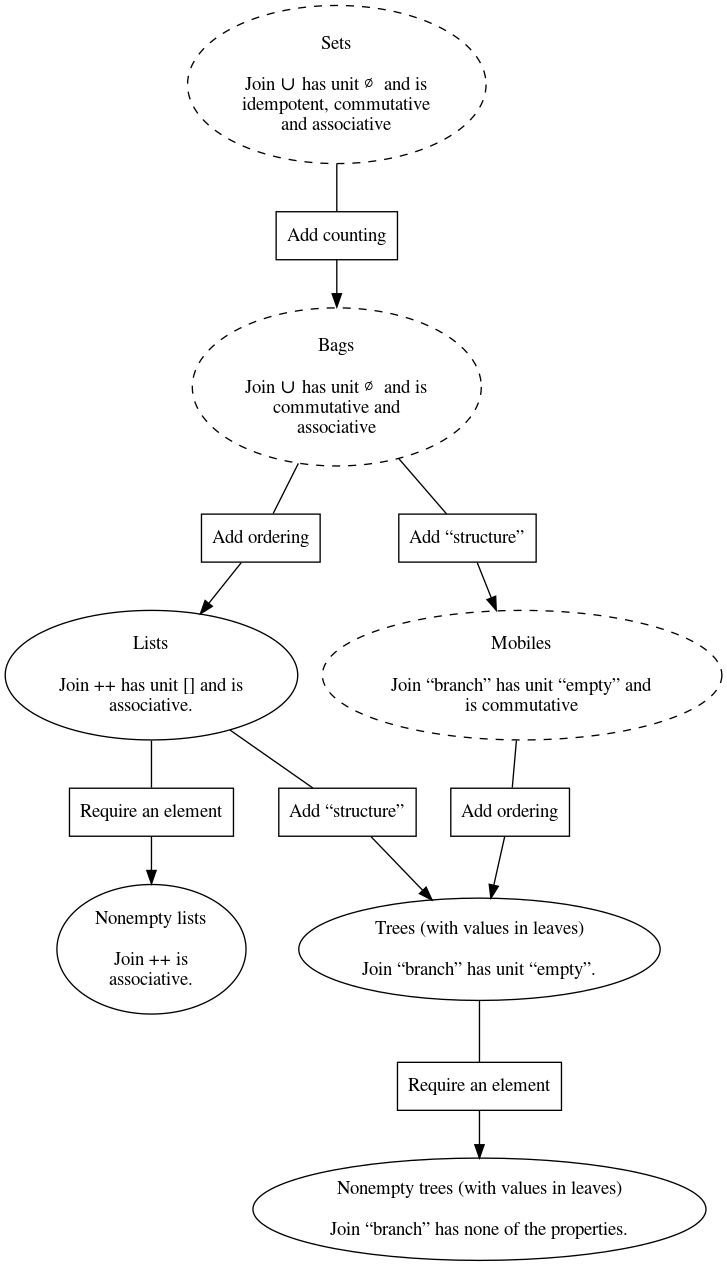
\includegraphics[width=\textwidth]{media/BOOM.png}
\end{center}

Not all of these types are easily representable in most programming languages;
we can say they are \emph{abstract} types instead of \emph{concrete} types.
I've highlighted the ones which are not in the diagram using dashed lines.

Exercise: Why are those types not easily represented in standard
programming languages?

Exercise: Is it impossible for those types to be easily represented
in a programming language?

\section{The Boom hierarchy in Scala\hfill{}\textsc{application}}
\label{sec:org8a88c76}
\begin{center}
\textbf{Heads up: this section consists of failed attempts}
\textbf{and subsequent corrections. Read carefully, and double check}
\textbf{before borrowing any code. Or skip to the next section.}
\end{center}

\subsection{The \texttt{AppendList} type}
\label{sec:org8c839c0}
Let us implement the list type as described in the Boom hierarchy paper
in Scala. We'll call these \texttt{AppendList}, as they take \texttt{Append} as
the basic operation.

\begin{center}
\textbf{Extra heads up: there's a big flaw in defining lists this way,}
\textbf{so even when we get it right we're wrong.}
\textbf{We'll discuss the problem at the end.}
\end{center}

Those lists have three cases;
\begin{itemize}
\item the \texttt{Empty} list,
\item the \texttt{Single}-ton lists, and
\item the \texttt{Concat}-enation of two lists.
\end{itemize}

The Scala convention for implementing such types
has us start with a super-type from which a type
for each case will be derived.
This super-type should not be instatiable,
because we want to restrict to a number of cases :TODO:.

A \texttt{trait} is similar to a \texttt{class}, except it cannot be instantiated.
It is similar to an \texttt{interface} in Java.
(This also makes it similar to an \texttt{abstract class},
except it's more flexible; see
\href{https://docs.scala-lang.org/overviews/scala-book/abstract-classes.html}{the Scala docs}.)
\begin{minted}[breaklines=true]{amm}
trait AppendList[A]
\end{minted}

\subsection{Attempt 1 at defining cases of lists: basic classes}
\label{sec:orge599669}
Now we need to add sub-types which are instantiable.
Then since every element of the sub-type is also an element
of the super-type, we can create elements of \texttt{List}.

As Scala is object oriented, this means we want
a class definition for each case.

We can jump right to it.
\begin{minted}[breaklines=true]{amm}
class Empty[A]() extends AppendList[A]
class Single[A](a: A) extends AppendList[A]
class Concat[A](l: AppendList[A], r: AppendList[A]) extends AppendList[A]
\end{minted}

But if we try out this definition, we may be disappointed.
\begin{minted}[breaklines=true]{amm}
val empty1 = new Empty[Int]
val empty2 = new Empty[Int]

val list1 = new Concat(new Single(1), new Single(2))

empty1 == empty2  // equality check
empty1.eq(empty2) // reference equality check
\end{minted}

\subsection{Attempt 2 at defining cases of lists: case classes}
\label{sec:orgc117080}
The reason why our classes above allowed multiple instances
of “the same” list is because, although we are not including any,
a regular \texttt{class} may have mutable data (non-constant fields).
So the runtime is aware that \texttt{empty1} and \texttt{empty2} could
actually be different (even though, with just our definitions above,
there isn't a way to make them significantly different).

When defining this sort of \emph{algebraic datatype} in a
functional style, we want \emph{immutability}, to ensure that
two objects which are constructed the same way
are in fact the same.

Scala provides \texttt{case} classes for this.
A \texttt{case} class has no mutable state (no non-constant fields),
and all its fields are public.
\begin{minted}[breaklines=true]{amm}
case class Empty[A]() extends AppendList[A]
case class Single[A](a: A) extends AppendList[A]
case class Concat[A](l: AppendList[A], r: AppendList[A]) extends AppendList[A]
\end{minted}

The name \texttt{case class} is used because,
given this immutable nature,
\emph{pattern matching} (or \emph{case splitting})
makes sense.

\subsection{The inherent problem with \texttt{AppendList}}
\label{sec:org7293ef1}
:TODO: discuss sealed

:TODO: no junk, no confusion

\begin{minted}[breaklines=true]{amm}
sealed trait AppendList[A]
case class Empty[A]() extends AppendList[A]
case class Single[A](a: A) extends AppendList[A]
case class Concat[A](l: AppendList[A], r: AppendList[A]) extends AppendList[A]

val x1 = Empty[Int]()
val x2 = Empty[Int]()
\end{minted}

\begin{minted}[breaklines=true]{amm}
val listofone = Single(1)
val anotherlistofone = Concat(listofone, Empty())

listofone == anotherlistofone
\end{minted}

\section{A proper implementation of lists in Scala.}
\label{sec:org8922f55}
\begin{minted}[breaklines=true]{elm}
type List a = Empty | Cons a (List a)
\end{minted}

Our final, correct implementation
\begin{itemize}
\item ensures there is only one way to construct a given (abstract) list,
by using more concrete constructors,
\item marks the \texttt{trait} as \texttt{sealed}, so no further constuctors may be added, and
\end{itemize}
\begin{minted}[breaklines=true]{scala}
sealed trait ConsList[A]
case class Empty[A]() extends ConsList[A]
case class Cons[A](hd: A, tl: ConsList[A]) extends ConsList[A]
\end{minted}

We can try out some definitions on this type.
\begin{minted}[breaklines=true]{scala}
def sum(xs: ConsList[Int]): Int = xs match {
  case Empty() => 0
  case Cons(hd, tl) => hd + sum(tl)
}

def append[A](xs: ConsList[A], ys: ConsList[A]): ConsList[A] =
  xs match {
    case Empty() => ys
    case Cons(hd, tl) => Cons(hd, append(tl, ys))
  }
\end{minted}

\begin{minted}[breaklines=true]{scala}
val test = Cons(1,Cons(2,Cons(3,Empty())))
val test2 = Cons(1,Cons(2,Cons(3,Empty())))

append(test,test2)
\end{minted}

\section{Reset the REPL!}
\label{sec:org5b179d5}
A nice feature of the Ammonite REPL for Scala
is that you can save and load the session state,
allowing you to more safely try things out
and then restore to an earlier state if you need to.
See \url{https://ammonite.io/\#Save/LoadSession}

To save, run
\begin{minted}[breaklines=true]{amm}
repl.sess.save()
\end{minted}

To load, run
\begin{minted}[breaklines=true]{amm}
repl.sess.load()
\end{minted}

Note you can provide strings as arguments to name the states
being saved/loaded.

If you don't use names, and need to restore an older state,
you can use \texttt{repl.sess.pop(n)} to pop \texttt{n} saved states off the session.

If you simply want to restart, just off an extreme number
of saved states.
\begin{minted}[breaklines=true]{amm}
repl.sess.pop(999)
\end{minted}

\section{Scratch}
\label{sec:orgcb5c03e}
\begin{minted}[breaklines=true]{amm}
case class test() {
  var x = 1
  def hello() = 1
}
\end{minted}
\end{document}
